A new semi empirical method to predict roll damping has been developed. The new method is based on regression of the present roll damping database together with some parts of the Simplified Ikeda method.  The regression was conducted on the roll damping database for tests at even keel (trim smaller than 0.4 degrees).

When looking at the roll damping database it was found that the roll damping at zero speed is much lower than the roll damping at speed. The hydrodynamics at zero speed and at speed is very much different \cite{ikeda_velocity_1979}. Because of this the regression has been divided as a product of two sub models:
\begin{equation} \label{eq:regression_factor_equation}
B_{e hat} = B_{e factor} B_{e hat 0}
\end{equation}

Where $B_{ehat0}$ is zero speed regression and $B_{efactor}$ is a speed depending regression. Linear regression has been used for the two sub models. 

\begin{figure}[H]
    \centering
    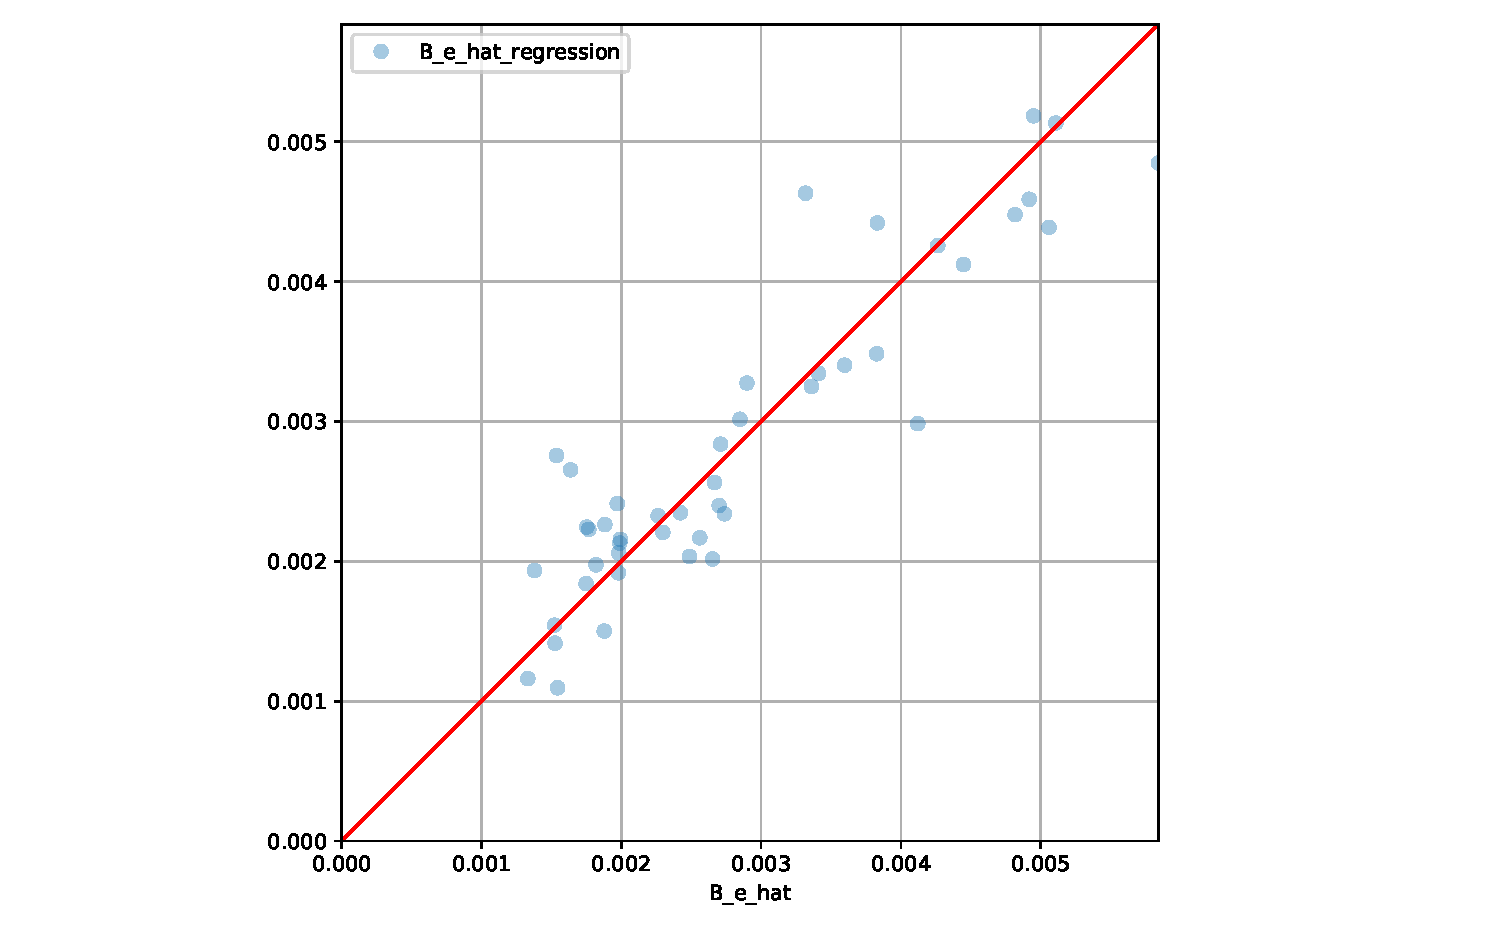
\includegraphics[width=\columnwidth]{figures/B_e_hat0_regression.pdf}
    \caption{Zero speed regression}
    \label{fig:B_e_hat0_regression}
\end{figure}
Figure \ref{fig:B_e_hat0_regression} shows a comparison between predictions with the zero speed model and the damping at zero speed from the database.

\begin{figure}[H]
    \centering
    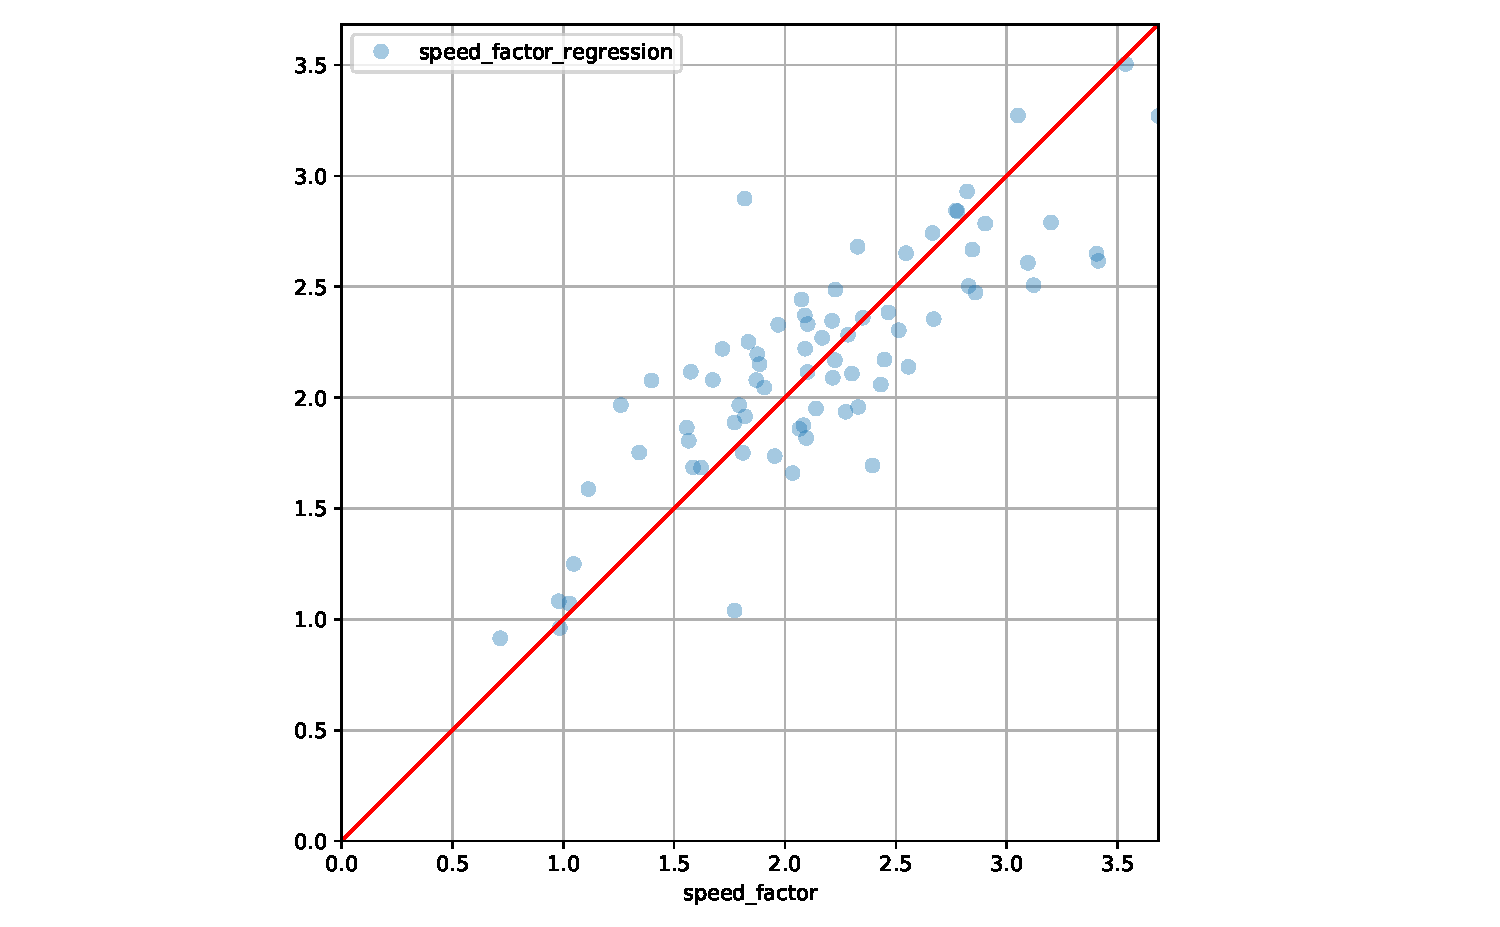
\includegraphics[width=\columnwidth]{figures/B_e_factor_regression.pdf}
    \caption{Speed dependency regression}
    \label{fig:B_e_factor_regression}
\end{figure}
Figure \ref{fig:B_e_factor_regression} shows a comparison of the speed dependence regression. It can be noted that the speed factor can be up to 3.5 so that the roll damping at speed is 3.5 times larger than the corresponding roll damping at zero speed.

\begin{figure}[H]
    \centering
    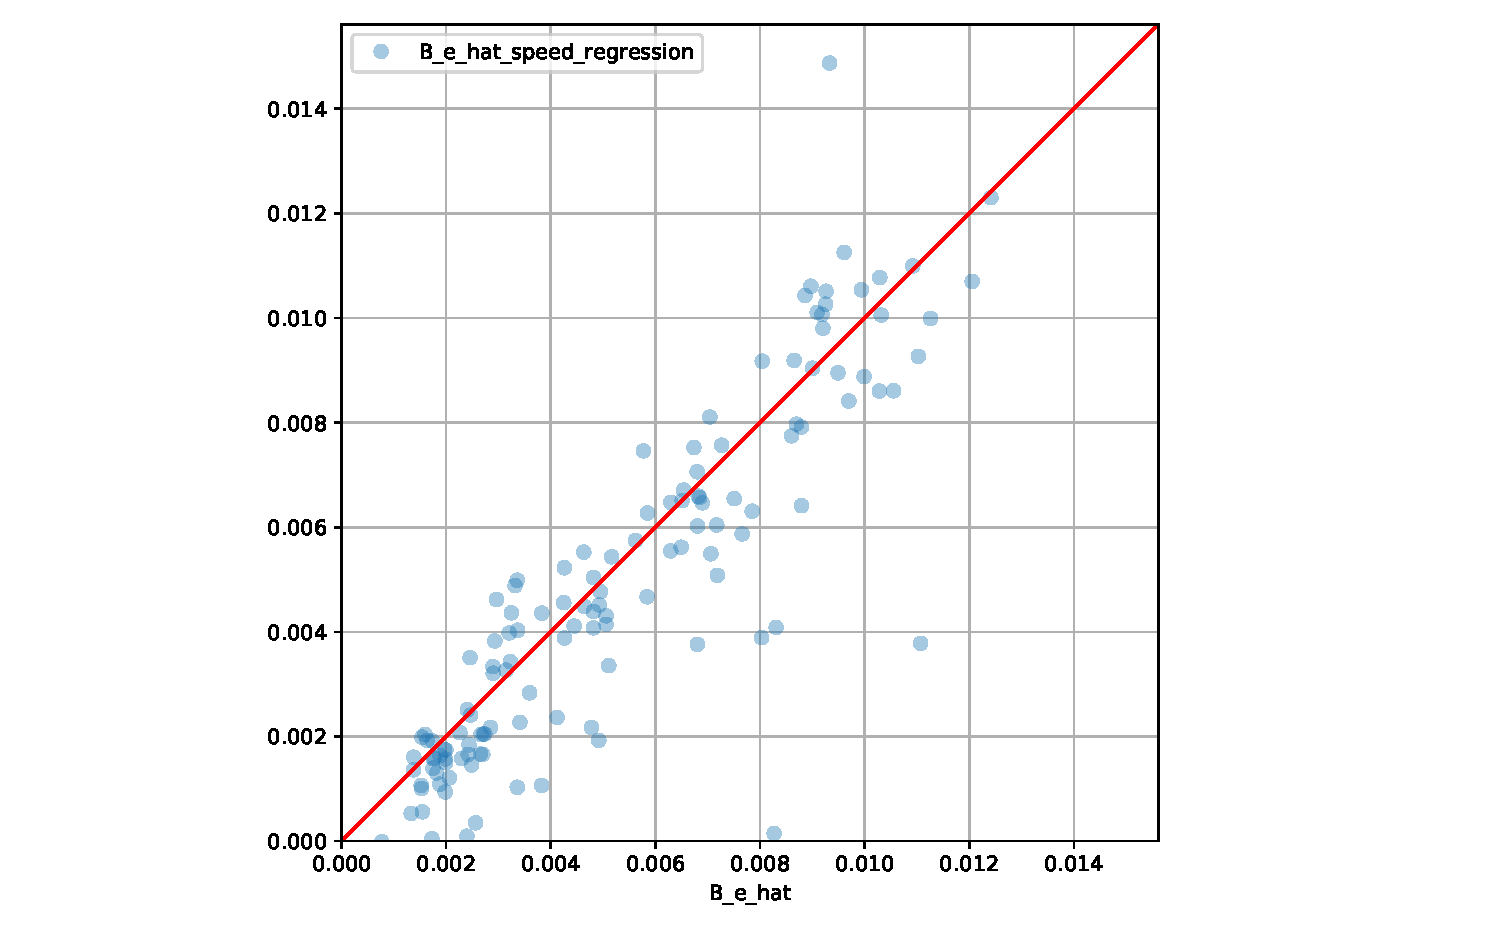
\includegraphics[width=\columnwidth]{figures/B_e_factor_regression_total.pdf}
    \caption{Total regression}
    \label{fig:B_e_factor_regression_total}
\end{figure}
Figure \ref{fig:B_e_factor_regression_total} shows a comparison between predictions with the total regression model (equation 
\ref{eq:regression_factor_equation}) and the whole roll damping database. The regressed sub models are shown in equation \ref{eq:polynom_zero} and \ref{eq:polynom_speed}. The non-dimensional damping due to hull lift $B_{LHAT}$, from the Ikeda method, is one of the parameters in the speed dependency equation \ref{eq:polynom_speed}.


\begin{equation} \label{eq:polynom_zero}
B_{e hat} = - 0.0136052800165908 A_{0} + 0.759326775676605 BK_{B} + 0.0725876320147426 GM - 0.0303297720484823 T + 0.00126493893040265 \omega_{0 hat} + 0.0143189616219315
\end{equation}

\begin{equation} \label{eq:polynom_speed}
B_{e factor} = 84.1 B_{L HAT} + 3.64 V + 0.468
\end{equation}


\subsection{Cross validation}
When constructing a regression model from a data set, over-fitting the data can be a problem. Including too many parameters and/or allowing too high order of the model would give a very good representation of the present roll damping data, but would generate large extrapolation errors when the model is used on other data. Cross validation has been used to "mimic" this situation where the model should make predictions on "new data", for ships that have not been part of the regression (the training of the model). The model that can make the best prediction on "new data" is considered as the best model. The best model has been developed by optimizing the selection of parameters, the features. The regression model was allowed to have features selected from a "gross list" of all available meta data. The linear regression should determine coefficients in a mathematical expression represented as a polynomial up to second order and including coupling terms. The model with a selection of terms that gives the highest score in the cross validation is considered as the best one.    

For the cross validation the data has been divided into a  training set (80\%) and a testing set (20\%). The selection has been made so that all tests with a specific ship model and its loading conditions are all in either the training set or the testing set. Only tests where there are results for both zero speed and speed (for the same loading condition and ship model) are included.

The "gross list" of available features has been chosen as a balance between guessed relevance and to minimize the number of tests that need to be excluded due to missing meta data. 
The number of parameters was also kept to a minimum so that a set of fewer features was selected prior to one with more features if they had similar scoring. As it turned out the developed regression models (equation \ref{eq:polynom_zero} and \ref{eq:polynom_speed}) have no coupling terms or quadratic terms.

The total regression model, consisting of the two sub models, was evaluated using cross validation. 100 random train/test sets were fitted and tested giving an average score: $mean(R^2)=0.66$, with standard deviation $std(R^2)=0.12$.